\documentclass[preprint]{elsarticle}

\usepackage{amssymb}
\usepackage{amsmath, amsthm}
\usepackage{amstext, amsfonts}
\usepackage{graphicx}
\usepackage{epstopdf}

\newcommand{\rf}[1]{(\ref{#1})}
\newcommand{\RR}{\mathbb{R}}
\newtheorem{thm}{Theorem}
\newtheorem{lm}{Lemma}
\newtheorem{cor}{Corollary}
\newdefinition{rmk}{Remark}

\newcommand{\dO}{\partial\Omega_{h}}

\def\ra#1{\renewcommand{\arraystretch}{#1}}
\def\ds{\displaystyle}
\def\bar#1{{\overline{#1}}}

\journal{Mathematics and Computers in Simulation}

\begin{document}

\begin{frontmatter}

\title{Numerical Study of Traveling Wave Solutions to 2D Boussinesq  Equation}


\author{K. Angelow\corref{cor1}}
\ead{angelow@mail.bg}
\author{N. Kolkovska}
\cortext[cor1]
{
Institute of Mathematics and Informatics, Bulgarian Academy of Sciences, Acad. G.~Bonchev Bl.8, 1113 Sofia, Bulgaria
}

\address{Institute of Mathematics and Informatics, Bulgarian Academy of Sciences, Acad. G.~Bonchev Bl.8, 1113 Sofia, Bulgaria}

\begin{abstract}
The aim of this paper is to evaluate stationary  propagating  wave solutions  
 to the two dimensional Boussinesq  equation. To solve the resulting nonlinear fourth order elliptic  problem we use a  combination of high order finite difference schemes, an iterative procedure  and  new asymptotic boundary conditions.   A number of numerical results are obtained for the validation of the method and for dependence of the wave's shape on the velocity $c$ and dispersion parameters. We give also a comparison with  the numerical results and best-fit formulae given in \cite{Ch2011,Ch2012}.

\end{abstract}
\begin{keyword}
two dimensional Boussinesq  equation \sep traveling wave solutions (TWS) \sep high order finite difference schemes \sep asymptotic boundary conditions
 \end{keyword}
\end{frontmatter}


\section{Introduction}\label{introduction}

In this paper we  consider the two dimensional Boussinesq  Equation (BE)
\begin{align}
&u_{tt} - \Delta u -\beta_1  \Delta u_{tt} +\beta_2 \Delta ^2 u + \Delta f(u)=0   \quad \text{for}  (x,y) \in \RR^2, \, t\in\RR^+,\label{eq1}
\\ \nonumber &u(x,y,0)=u_0(x,y), \, u_t(x,y,0)=u_1(x,y)   \quad\text{for} \, (x,y) \in \RR^2,
\\  &u(x,y) \rightarrow 0,  \Delta u(x,y) \rightarrow 0 ,  \quad \text{for}  \sqrt{x^2 + y^2} \rightarrow \infty, \label{eq11}
\end{align}
where   $f(u)=\alpha u^2$,  $\alpha>0$, $\beta_1>0$, $\beta_2>0$  are dispersion parameters, and $\Delta$ is the Laplace operator. The BE is famous with the approximation of shallow water waves or also weakly non-linear long waves. It is oftern used for simulation of various physical processes e.g. turbulence in fluid mechanics, vibrations in acoustics and, etc. A derivation of the BE from the original Boussinesq system can be found in \cite{ChChr}.

The goal of the article is to to seek for solutions to (\ref{eq1}) of the type $u(x,y,t)=U(x,y-ct)$, which 
are stationary solitary waves (SSW) traveling  in $y$ direction with velocity $c$. In a forthcoming paper the SSW will be applied as initial condition (IC) of the hyperbolic BE \rf{eq1}, \rf{eq11}. Thus it is useful to have accurate, flexible 
and robust IC in order to test various scenarios with two or more traveling waves colliding with each other.

The SSWs to \rf{eq1} are computed by a Galerkin spectral method in \cite{chr-chr-07,chr-chr}.
In \cite{Ch2012} a second order  finite difference scheme is used, while in \cite{Ch2011} 
the perturbation series method with respect to the small parameter $c$ is applied.  Moreover in \cite{Ch2011} 
the resulting numerical solution is approximated by best-fit formulae. These exact expressions are used further as initial conditions in 
numerical simulations of the unsteady BE \rf{eq1}-\rf{eq11}, see  \cite{cher,dani}. It is shown in these papers, 
that for velocities $c<0.3$ the resulting SSW disperse in the form of ring wave expanding to infinity or blow up after some period in time. 
Thus the traveling wave solutions of the hyperbolic equation  \rf{eq1} are very fragile, i.e. the wave easily blow up or fall apart with time. 
The relationship between the dispersion and nonlinearity in \rf{eq1} is very sensitive  and the balance between them is easily destroyed.
Moreover it is well known  that in the one dimensional case the solitary waves are unstable  
for small wave speeds $c$ while they are stable in form for  velocities $c$ close to $1$. 


Having in mind these  observations, we focus in this paper on the more accurate evaluation of SSW $U$ to \rf{eq1}, especially for  velocities $c > 0.7$, since it is fundamental for the construction of initial data of the unsteady BE \rf{eq1}. 

Note that the stationary solitary waves $U(x,y-ct)=u(x,y,t)$
 satisfy the following nonlinear fourth order elliptic equation

\begin{equation}\label{eq2}
c^2 (E-\beta_1 \Delta) U_{yy} = \Delta U -\beta_2 \Delta^2 U - \Delta f(U),
\end{equation}
where $E$ is the identity operator. 

The evaluation of the solution to \rf{eq2} described here follows the steps presented in \cite{Ch2012},
but new modifications are introduced to meet the higher requirements reported above.

First, for the numerical solution of \rf{eq2} we choose to apply an uniform grid with equal step size $h_x$ = $h_y$ = $h$ in the computational domain $\Omega_h$ instead of an nonuniform grid. The reason for this is that  
%
%because of the following circumstances. 
 the computed solutions to \rf{eq2} will be used as initial conditions in the hyperbolic problem \rf{eq1} and these solutions will travel in time, thus we have to have more mesh points not only close to the peak of the waves, but everywhere in   the  computational domain. 

In order to increase the precision of the numerical method, we apply finite difference schemes (FDS) with local approximation of forth $O(h^4)$ and sixth $O(h^6)$ order, i.e. we  approximate second order spatial derivatives with high order finite differences. These  FDS allow one to evaluate the numerical solution with high accuracy on relatively coarse grid. 

A new boundary condition on the computational boundary is also used, together with uniform grid and local approximation order of $O(h^4)$ and $O(h^6)$. The numerical solution of the fourth order elliptic problem \rf{eq2} is replaced with an iterative procedure, which involves solution  of an appropriate  parabolic type problem at every iteration step. %until this solution converges. 
%It is emphasized here that elliptic solutions and combinations of those are used in the hyperbolic problem, e.g. wave collision. There are at least two moving peaks when a combination is used. The numerical grid $\Omega_h$ could be chosen with more points near the peak and less points near the boundary, i.e. use non-uniform grid. But as long as the numerical simulation for the hyperbolic equation requires more than one wave which travels at larger distances (much larger than the discretization step) the straightforward and easiest approach is to use uniform grid with equal step size $h_x$ = $h_y$ = $h$. In order to increase the precision, the numerical method here uses local approximation of forth and sixth order $O(h^4)$ and $O(h^6)$. The high order finite difference schemes (FDS) allow to evaluate the numerical solution with high accuracy on relatively coarse grid.
%Recall that in the one dimensional case the BE possesses well known solitary wave solutions of 'sech' type, see \cite{Ch1996}. 
%The  TWS to \rf{eq1} in the two dimensional case  were  computed in \cite{chd-chr, chr-chr-07,chr-chr,Ch2011,Ch2012}. 
%Thus the accurate evaluation of the solutions to \rf{eq2} is fundamental for the construction of initial data of the unsteady BE where the focus is on wave speeds $c > 0.7$. 
 %A new boundary condition is used, together with uniform grid and local approximation order of $O(h^4)$ and $O(h^6)$. The application of high order finite difference schemes (FDS) allows on to evaluate the numerical solution with high accuracy on relatively coarse grids. 
At the end of each iteration procedure the residual (17) of the discrete equation, approximating (4) is of order $10^{-5}$, $10^{-6}$ and the distance between two consecutive iterations of the solution is of order $10^{-7}$, which is much smaller than the discretization step size $h$.
 
In the last section we examine the solution shape and the dependence of the solution on the input  parameters - the velocity $c$ and the relative dispersion $\beta =\beta_1  / \beta_2$. We show that these  qualitative properties of the numerical solution are very similar to those given for the  numerical solution in \cite{Ch2011,Ch2012}. 
We compare our results with the best-fit  (approximating the numerical solution)  formulas stated in \cite{Ch2011}.   
The analysis  shows that  these best-fit formulas do not satisfy the equations in the neighborhood of the origin in the classical sense because their fourth order derivatives have singularities at the origin.  The  difference (measured in the maximal norm and in $L_2$ norms)  between our numerical solution and the corresponding best-fit formulae is also high, especially  for large velocities $c$. 

The paper is organized as follows. In Section~2 we formulate the  problem. The numerical method is given in Section~3 and validated in Section~4.  Various numerical  experiments and a comparison with  results in \cite{Ch2011,Ch2012} are reported in Section~5.

\section{General Formulation}

By the change of variables $x=\sqrt\beta_1 { \overline x}$, $y=\sqrt\beta_1 { \overline y}$, $U(x,y)= v({ \overline x},{ \overline y} )$ 
 equation \rf{eq2} is rewritten in the form 
 \begin{equation}\label{eq3}
c^2 \beta (E- \Delta) v_{{\overline y}{\overline y}} = \beta \Delta v - \Delta^2 v - \beta \Delta f(v)
\end{equation}
with   $\beta = \beta_1 / \beta_2$.
The solution $v$ to \rf{eq3} and its derivatives  tend to zero as $|x^2 +y^2|\rightarrow \infty$.
In the following we use notations $x,y$ instead of ${\overline x},{\overline y}$.

If the condition $c^2 < \min (1/ \beta,1)$ holds then  \rf{eq3} is an elliptic equation of fourth order and the linear second order derivatives in \rf{eq3} form  a second order elliptic equation. In this paper we consider velocities $c$ which fulfill this inequality.

Problem \rf{eq3} can be rewritten  as a  system of two elliptic equations of second order in different ways. We expect that  the derivatives $v_{xx}$ in $x $ direction  will be smaller than the derivative $v_{yy}$ in $y$ direction (since the solution travels in $y$ direction). Therefore the equality $v_{yy} = \Delta v- v_{xx}$ is substituted in \rf{eq3} and, after  introducing an auxiliary  function $w$, we obtain the equivalent to \rf{eq3} system
\begin{equation}\label{eq4}
- (1-c^2 \beta) \Delta v + \beta (1-c^2) v + \alpha \beta v^2 = w, 
\end{equation}
\begin{equation}\label{eq44}
 - \Delta w =  c^2 \beta (E- \Delta) v_{xx}. 
\end{equation}
We  seek  non-trivial solutions to \rf{eq4}-\rf{eq44}. To avoid the trivial solution we proceed as in \cite{Ch2012}: we fix the value of the solution $v$ at the point $(0,0)$,    $v(0,0)=\theta $ and introduce  new  functions: $\widehat{v}=v/{\theta} $ and $\widehat{w}=w/{\theta} $. Thus  
$ \widehat{v}(0,0)=1$ and 
\begin{equation}\label{eq45}
\begin{split}
 - (1-c^2 \beta) \Delta \widehat{v} + \beta (1-c^2) \widehat{v} + \alpha \beta \theta \widehat{v}^2 = \widehat{w}, \\
 - \Delta \widehat{w} =  c^2 \beta (E- \Delta) \widehat{v}_{xx}.\;\;\;\; \;\;\;\;  \;\;\;\;  \;\;\;\; 
\end{split}
\end{equation}
The value of $\theta $ is found from the  equation 
\begin{equation}\label{eqtheta}
\theta = \frac{ (1-c^2 \beta) \Delta \widehat{v} - \beta (1-c^2) \widehat{v} +\widehat{w}}{\alpha \beta} |_{x=0,y=0} .
\end{equation}
In order to evaluate numerically the solution to \rf{eq45} we introduce artificial time, add false  time derivatives and  get
\begin{align}\label{eq5}
\begin{split}
 \frac {\partial \widehat{v}}{\partial t} - (1-c^2 \beta) \Delta \widehat{v} + \beta (1-c^2) \widehat{v} + \alpha \beta \theta \widehat{v}^2 = \widehat{w}, \\
 \frac {\partial \widehat{w}}{\partial t} - \Delta \widehat{w} =  c^2 \beta (E- \Delta) \widehat{v}_{xx}. \;\;\;\;  \;\;\;\;  \;\;\;\;  \;\;\;\;
\end{split}
\end{align}
Thus the solution to the steady coupled elliptic system \rf{eq45} is replaced by   solving the  pertinent transient equations \rf{eq5} until their solutions $\widehat{v}$ and $\widehat{w}$ cease to change significantly in time. 

\section{Numerical Method}

We  turn  to the numerical approximation of the   system \rf{eq5} discussed in the previous section. The backbone of the  algorithm is  described in \cite{Ch2012}. The following  improvements have been made in this article:   more accurate finite difference schemes of fourth and sixth order of approximation are applied and new type of  conditions on the external computational boundary are developed.

\subsection{Finite difference schemes}
First we replace the unbounded domain by a sufficiently large computational domain $\Omega$. Due to the obvious symmetry of the problem, we can look for the solution only in the first quadrant $\Omega = [0,L_x] \times[0,L_y]$. Then a uniform grid $\Omega_h$ is defined in the following way
$$
\Omega_h = \{(x_i,y_j): x_i = ih, y_j = jh, i = 0,\cdots ,N_x, j = 0,\cdots , N_y \},
$$
where the discretization step $h$ satisfies
$ h = L_x/N_x = L_y/N_y$. 
 In the  implementation of the numerical method
the  step size $\tau$ may vary according to the residual of the computed solution. This is a crucial point because it permits  to automatize the control of the error.
The value of the function $v$ at mesh point $x_i,y_j,t_k$ is denoted by $v_{i,j}^k$.

We discretize the spatial  derivatives in \rf{eq5} using centered finite differences  
and extending the stencil:
\begin{equation}\label{fd}
v_{\widehat{xx},p}(x) :=  \frac{1}{h^2} \sum\limits_{i=-p/2}^{p/2} d_i v(x+ih),
\end{equation}
 Here $p$ is equal to $2$, $4$ or $6$.  The weights $d_i$ taken from  \cite{forn} are  
 $ 1,-2,1$ for $p=2$, $-\frac{1}{12}, \frac{4}{3}, -\frac{5}{2}, \frac{4}{3}, -\frac{1}{12}$ - for $p=4$ and  $\frac{1}{90}, -\frac{3}{20}, \frac{3}{2}, -\frac{49}{18}, \frac{3}{2}, -\frac{3}{20}, \frac{1}{90}$ - for $p=6$. The approximation error of  formulae \rf{fd} is $O(h^p)$. Replacing the Laplace operator in \rf{eq5} by the discrete Laplacian $$ \Delta_{h,p} v_{i,j} := (v_{i,j})_{\widehat{xx},p} + (v_{i,j})_{\widehat{yy},p}$$ we obtain finite difference schemes with high order of approximation $O(h^4)$ for $p=4$ and  $O(h^6)$ for $p=6 $.  The application of FDS with high order of approximation leads to a high rate of convergence of the method for   sufficiently smooth solutions.
In this way more accurate solutions can be produced on a coarse grid.

Symmetry conditions are used to impose the values of the discrete Laplacian at mesh points close to ${(0,y)}$, and $(x,0)$. 
Near  the computational boundaries $(x,y):x=L_x$ and $(x,y):y=L_y$ we do not change the stencil. The discrete Laplacian
is defined  there by using the values of the discrete solution given in \rf{bFunV}, \rf{bFunW} below at  points outside the computational domain.

\par
The Euler explicit rule is applied for approximation of  time derivatives. The nonlinear terms in \rf{eq3} are computed on    time level $t^k$. Thus, the numerical solutions at time level $t^{k+1}$ are evaluated directly by the values of the numerical solution at time level $t^k$:  
 \begin{equation}\label{eq55}
 \begin{split}
   \frac {\widehat{v}_{i,j}^{k+1}-\widehat{v}_{i,j}^{k}}{\tau}- (1-c^2 \beta) \Delta_{h,p} \widehat{v} _{i,j}^{k}+ \beta (1-c^2     ) \widehat{v}_{i,j}^{k} + \alpha \beta \theta (\widehat{v}_{i,j}^{k})^2 = \widehat{w}_{i,j}^{k}, \\
  \frac  {\widehat{w}_{i,j}^{k+1} -\widehat{w}_{i,j}^{k}} {\tau} - \Delta_{h,p} \widehat{w}_{i,j}^{k} =  c^2 \beta (E- \Delta_{h,p})       
    \widehat{v}_{i,j,{\widehat{xx},p}}^{k}. \;\;\;\; \;\;\;\;\;\;\;\;\;\;\;\;
\end{split}
\end{equation}
This method for solving equations 
\rf{eq45} can be considered also as ``the simple iteration method'' for solving linear and nonlinear equations (see \cite{sam}).


\begin{rmk}\label{R1}
It is possible to use varying time step $\tau$ to optimize and speed up the algorithm. When the time step becomes too big the solution starts to diverge and becomes jagged. Fortunately these signs appear first in the residual i.e. it
starts to grow and jag simultaneously while the solution is still fine. 
Arbitrary cross-sections of the residual look like a discrete function
which alternates positive with negative values on the grid.
This is a clear sign that the time step has to be decreased, otherwise we can increase it.
\end{rmk}
 In order to start the procedure we need initial values for functions $\widehat{v},\widehat{w}$. These initial values are taken from the  formulae in \cite{Ch2011}.
 
\subsection{Asymptotic conditions on the  boundaries $x=L_x$ and $y=L_y$}

The behavior of the solutions $v$ and $w$  as $r =\sqrt{x^2 +y^2} \rightarrow \infty$ is studied in details in \cite{Ch2011,Ch2012}. From the numerical results  given there it follows that   $v$ and $w$ have $O( r^{-2})$ asymptotic decay at infinity. We suppose that the  second order derivatives of $v$ and $w$  are of order $O(r^{-4})$  whereas  fourth order derivatives and the nonlinear term in equation \rf{eq3}   are of order $O(r^{-6})$.
These assumptions 
help us to evaluate the solution  on the outer computational boundary $B= \{(L_x,y):0\le y\le L_y\} \cup \{(x,L_y):0\le x\le L_x\} $. 

Consider equation \rf{eq3} for  sufficiently large $r$. 
 We insert the asymptotic values of all terms  in \rf{eq3} and  neglect the higher order in $r$ terms  (of order $O(r^{-6})$). In this way we obtain the  following  problem  valid for large $r$ 
\begin{subequations}\label{asympt}
\begin{align}
c^2 v_{yy} &= \Delta v, \label{one}
\\
v(x,y),  \Delta v(x,y) &\rightarrow 0~ \mbox{as}~ \sqrt{x^2 + y^2} \rightarrow \infty. \label{two}
\end{align}
\end{subequations}
The  function that resolves   equations \rf{one} and \rf{two} is
\begin{equation}\label{sol}
\begin{split}
v (x,y)=
 \mu ( (1-c^2)x^2+y^2 )^{-q/2}
\cos(q \: \arccos(\frac{\sqrt{1-c^2} x }{ \sqrt {(1-c^2)x^2 + y^2} }))
\end{split}
\end{equation}
with  some positive real numbers $\mu$ and $q$. 
Using the asymptotic decay of the solution and its symmetry with respect to coordinate axes,   we obtain  $q=2$ and simplify  \rf{sol}  to
\begin{equation}\label{bFunV}
\bar{v}(x,y) = \mu \frac{( (1-c^2)x^2-y^2 )}{((1-c^2)x^2 + y^2)^2 }.
\end{equation}

Similar considerations for the function $w$ and equation \rf{eq4} lead to an expression that substitutes $w$, valid for  large $r$ 
\begin{equation}\label{bFunW}
\bar{w}(x,y) =\tilde {\mu} (1-c^2) \frac{( (1-c^2)x^2-y^2 )}{((1-c^2)x^2 + y^2)^2 },
\end{equation}
with a new unknown parameter $\tilde {\mu}$. 

In order to resolve the boundary functions \rf{bFunV} and \rf{bFunW} completely one needs $\mu$ and $\tilde {\mu}$ parameters.
We obtain them iteratively, at each time level of \rf{eq55}, by the following minimization procedure. For  given solutions  $v^k_{i,j}$ and $ w^k_{i,j}$ at time level $t^k$ 
we choose $\mu$ and $\tilde {\mu}$ as minimizers of 
\begin{equation}\label{mu}
\begin{split}
\mu = \underset{\mu>0 }{\operatorname{min} } \| \bar{v}(x_i,y_j) - \widehat{v}^k_{i,j} \|_{L_2,\widehat{\Omega}},
\;\;
\tilde {\mu} = \underset{\mu>0 }{\operatorname{min} } \| \bar{w}(x_i,y_j) -\widehat{w}^k_{i,j} \|_{L_2,\widehat{\Omega}}.
\end{split}
\end{equation}
Tests and simulations showed that $ \widehat{\Omega} $ should not solely consist of boundary points but should also include some inner points of $\Omega_h$ near boundary $B$.
Each minimization problem produces a simple linear equation, which depends on the type of norm used in \rf{mu}. 

Validation of this part of the numerical algorithm is given in Subsection~4.2. 

\subsection{Stop Criteria}

Usually  the calculations of  $\widehat{v}^{k+1} $ by equations \rf{eq55} are  terminated if
\begin{equation*}
\max_{i,j} |\widehat{v}^{k+1}_{i,j}-\widehat{v}^{k}_{i,j}| < \epsilon \max_{i,j} |\widehat{v}^{k}_{i,j}| ,
\end{equation*}
where $\epsilon $ is a prescribed accuracy. 
Our numerical computations show that 
$$
\max_{i,j} |\widehat{v}^{k+1}_{i,j}-\widehat{v}^{k}_{i,j}| < \max_{i,j} | R_{i,j}^k |,
$$
where $R^k_{i,j}$ is the residual of the discrete approximation to \rf{eq3} at the mesh point $(x_i,y_j,t^k)$:
\begin{equation}\label{residual}
R_{i,j}^k := 
c^2\beta (\widehat{v}^k_{i,j})_{\widehat{yy},p} + \Delta_{h,p}(-\beta \widehat{v}^k_{i,j} - c^2\beta (\widehat{v}^k_{i,j})_{\widehat{yy},p} + \Delta_{h,p} \widehat{v}^k_{i,j} 
+ \alpha \beta \theta (\widehat{v}^k_{i,j})^2  ).
\end{equation}
Therefore we
apply the more restrictive criteria
\begin{equation}\label{stopCrit}
\max_{i,j} | R_{i,j}^k | < \epsilon \max_{i,j} |\widehat{v}^{k}_{i,j}|
\end{equation}
as  the  stop criteria of the procedure \rf{eq55}.  
In the implementation of the method  parameter $\epsilon$ is chosen to be $10^{-5}$ or $ 10^{-6}$.

\subsection{Basic algorithmic steps}
The following are the most important mile-stones during the implementation of the algorithm.
\\
1) Resolve proper initial condition $(v^0, w^0)$ on the grid $\Omega_h$.  Set parameters $\epsilon$ and $\tau$.
\\
2) Suppose $(v^k, w^k)$ are known. 
\par
2.1) Find current $\theta_k$ from the discrete approximation of \rf{eqtheta};
\par
2.2) Find current  parameters $\mu$ and $ \tilde{\mu}$ by minimizing expressions \rf{mu};
\par
2.3) Evaluate $\Delta_{h,p}  \widehat{v}^k$ and $\Delta_{h,p}  \widehat{w}^k$;
\par
2.4) Calculate $(\widehat{v}^{k+1}, \widehat{w}^{k+1})$  on the  time level $t^{k+1}$ by the Euler explicit scheme   \rf{eq55};
\par
2.5) Calculate the residual $R^{k+1}_{i,j}$ from  \rf{residual} and check the stop condition \rf{stopCrit}.
\par
2.6) Reduce or repeat the time step size $\tau$  (see Remark~\ref{R1}). Set $t^{k+1}=t^{k}+\tau$.
 
3) Continue steps 2.1) -2.6) with the next time level $t^{k+1}$ till condition \rf{stopCrit} is satisfied.

\section{Validation}\label{validation}

In this section we give several numerical results concerning the verification of  the presented numerical method. 
 We use FDS with different approximation errors and several sets  of  parameters $c$, $\alpha$, $\beta$,  which are shown on each table. 

 \subsection{Validation of the convergence of the numerical solution}\label{val-conv}
\begin{center}
\begin{table}[ht]
\centering
		\begin{tabular}{||c|l|ll|ll||}
			\hline
			\hline
      FDS       & $h$ &errors $E_i$in$L_2$&Conv. Rate& errors $E_i$in$L_\infty$&Conv. Rate\\
   			\hline 
					\hline 
      c=0.45    &0.2    &             &            &           &   \\
   $O(h^2)$     &0.1    &~ 0.037705  &            &~0.024736 &   \\
                &0.05   &~ 0.008922  &2.0794  &~0.005810 & 2.0901 \\
               	 \hline 
     c=0.1      &0.2   &             &           &                & \\
     $O(h^2)$   &0.1   &~ 0.015770  &             &~0.015794      &    \\
                &0.05  &~ 0.004854 & 1.6999       &~0.005243      & 1.5908  \\
			\hline
			\hline 	
      c=0.45    &0.2   &            &            &             &    \\
       $O(h^4)$ &0.1   &~ 0.020795   &           &~0.008505  &   \\
                &0.05  &~ 0.000278 & 6.2269    &~0.000235  & 5.1800  \\
					  			\hline 	
     c=0.1      &0.2  &            &               &               &     \\
     $O(h^4)$  &0.1   &~ 0.000892  &              &~0.001463      &        \\
               &0.05  &~ 5.4667e-05&4.0281        &~9.5747e-05 &  3.9337        \\
			\hline
    \hline
   c=0.45       &0.4   &            &        &                  &      \\
     $O(h^6)$   &0.2   &~ 2.0975e-02 &           &~2.9341e-02      &       \\
     &0.1  &~ 3.5348e-04 &5.8909  &~5.8346e-04 & 5.6521         \\
	  \hline
   c=0.1       &0.4   &             &        &               &        \\
     $O(h^6)$  &0.2   &~ 3.7059e-03  &        &~3.7572e-03     &       \\
   &0.1  &~ 7.4723e-05 &5.6321  &~8.3359e-05&   5.4942       \\
	   \hline
			\hline 
		\end{tabular}
		\caption{Convergence test for  FDS with different approximation errors. Errors $E_i$ are measured in $L_2$ and $L_\infty$ norms}

\label{tab:a}
\end{table}
\end{center}
 In this series of tests we evaluate the numerical solution of \rf{eq5} using FDS with approximation errors $O(h^2)$, $O(h^4)$, $O(h^6)$ and parameters  
 $\alpha = 1$,   $\beta=3$,  $\epsilon = 10e-5$, 
$L_{x }= 30$, $L_{y} = 30$.
The initial conditions for the artificial parabolic problem \rf{eq55} are taken from  \cite{Ch2011}. 
Using the values of numerical solution on three nested meshes we compute the numerical rate of convergence (Conv. Rate) in $L_2$ and $L_{\infty}$ mesh norms
by Runge method as $(\log E_1 -\log E_2)/\log 2$.  Here  $v_{[h]}$, $v_{ {[h/2]}  }$ and  $v_{ {[h/4]}  }$ represent the numerical solution over three nested meshes and $E_1=\|v_{[h]}-v_{[h/2]}\|$ , $E_2=\|v_{[h/2]}-v_{[h/4]}\|$.  
Table~\ref{tab:a} contains the errors in $L_2$ and $L_{\infty}$ norms and the corresponding numerical rate of convergence for the numerical solutions obtained by FDS with second, fourth and sixth order of approximation and   velocities  $c=0.1$  or $c=0.45$.
We observe that the experimental rate of convergence approximates well the approximation error of the difference schemes- the FDS are of  almost the same order of convergence as the order of approximation. An additional observation  is that  for  the same step size $h$ the schemes with higher order of approximation ($O(h^4)$, $O(h^6)$) lead to a more precise solution than the scheme with $O(h^2)$ approximation error. 


\subsection{Validation of the new boundary conditions}

Two tests are made to verify the new  conditions on the computational boundary $B$. The first one checks important parameters of  the numerical procedure from Subsection~3.2. In Table~\ref{tab:b}  the following quantities are presented at the end of the iteration procedure \rf{eq55}  for several computational domains $L_x=L_y=20, 40, 80, 160$ : the values of the solution $v$ at the point $(0,N_y)$; parameters $\mu$,  $\tilde{\mu}$ and the norms $\|v-\bar{v}\|_{2,\hat{\Omega}}$, 
$\|w-\bar{w}\|_{2,\hat{\Omega}}$, included in the minimization procedure \rf{mu}.  The initial problem is solved with  parameters  $\alpha = 1$, $\beta = 3$, $c = 0.45$, $\epsilon = 1.0e-05$, $h = 0.5$.
 \begin{center}
\begin{table}[ht]
\centering
		\begin{tabular}{||c|c|cc|cc||}
			\hline
			\hline
$L_x=L_y$&$v_{0,N_y}$& $\mu$&$\tilde{\mu}$&$\|v-\bar{v}\|_{2,\hat{\Omega}}$&$\|w-\bar{w}\|_{2,\hat{\Omega}}$ \\
	\hline		
              20&-2.23e-04 &1.9355e-01&1.9353e-01&~4.17e-05&~9.75e-05 \\
              40&-5.65e-05 &1.9370e-01&1.9369e-01&~4.42e-06&~1.03e-05 \\
              80&-1.41e-05 &1.9378e-01&1.9378e-01&~7.56e-07&~1.79e-06 \\
            160&-3.53e-06 &1.9381e-01&1.9381e-01&~7.44e-10&~1.40e-09 \\
   \hline
	\hline
		\end{tabular}
		\caption{Characteristic parameters of the minimization procedure \rf{mu} for different computational domains}
\label{tab:b}
\end{table}
\end{center}
The results in Table~\ref{tab:b} demonstrate that  parameters $\mu$ and $\tilde{\mu}$  converge as the domain becomes larger. The values of  $v$ (shown in the second column in  Table~\ref{tab:b}) decay with a rate of $1/r^2$. 

\begin{figure}[ht]
	\begin{minipage}[b]{0.5\linewidth}
		\raggedleft
		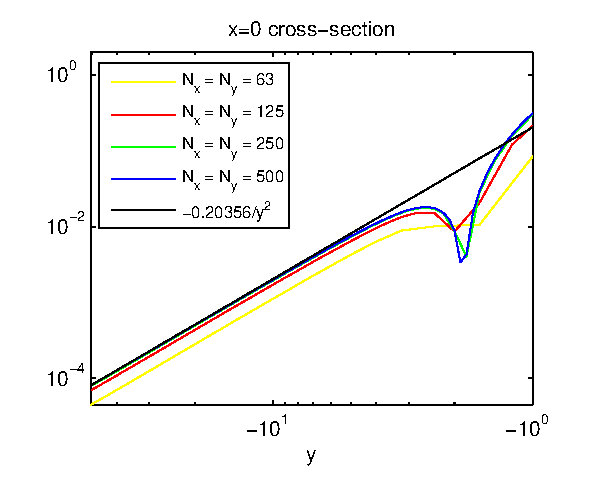
\includegraphics[width=\linewidth]{cross-sections/crossSectionLogX=0.eps}
	\end{minipage}	
	\begin{minipage}[b]{0.5\linewidth}
		\raggedright
		 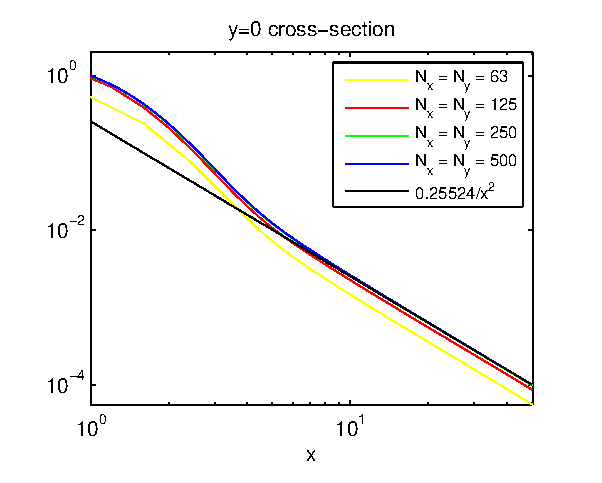
\includegraphics[width=\linewidth]{cross-sections/crossSectionLogY=0.eps}
	\end{minipage}
	\begin{minipage}[b]{0.5\linewidth}
		\raggedleft
		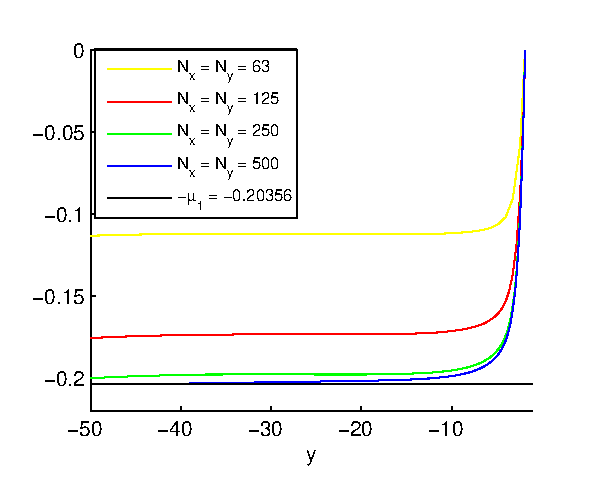
\includegraphics[width=\linewidth]{cross-sections/crossSectionX=0.eps}
	\end{minipage}	
	\begin{minipage}[b]{0.5\linewidth}
		\raggedright
		 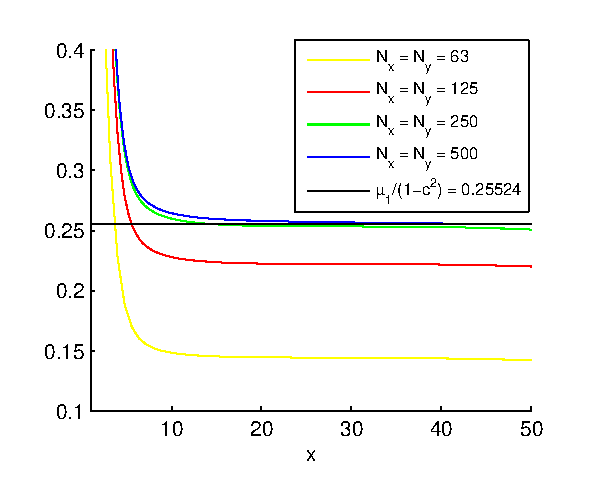
\includegraphics[width=\linewidth]{cross-sections/crossSectionY=0.eps}
	\end{minipage}
	\caption{The effect of the mesh size. Upper panels: the function. Lower panels: the function scaled by $r^2$.}
	\label{crossSections}
\end{figure}

The second test reveals the asymptotics of the numerical solution presented in log-log plots. 
 Pictures in Figure~\ref{crossSections} demonstrate important aspects of solution's cross sections on four different grids. The size of the computational domain $[0,50]\times [0,50]$ is kept constant and only the step $h$ changes,
$h = 0.1, 0.2, 0.4, 0.8$. We set the following parameters:  $\alpha = 1$, $\beta = 3$, $c = 0.45$, $\epsilon = 1.0e-05$.

 The first two horizontal pictures in Figure~\ref{crossSections} present logarithmic scaled plots of the absolute value of the numerical solution $v$. One can see the 
 decay $1/r^2$ at infinity guided by the black line. The next two horizontal pictures show the numerical solution scaled by a factor $r^2$. Thus these graphs display $v r^2$ along the vertical $z$ axis. One can observe that the scaled profile of the solution approximates a constant for large values of $r$. 
These plots are in  agreement with the new boundary function $\bar{v}$ found in \rf{bFunV} and with the asymptotics  of the solution. 
 Further using equation \rf{bFunV} for $x=0$ or for  $y=0$ one has for sufficiently large $r$ 
\begin{equation*}
\bar{v}(0,y) = -\frac {\mu} {y^2}, \ \ \  \bar{v}(x,0) =\frac {\mu} {(1-c^2)x^2},  
\end{equation*}
which explains the connection between the two constants displayed on the left part of Figure~\ref{crossSections} and the right part of right Figure~\ref{crossSections} legends.
All graphs in Figure~\ref{crossSections} show that the solution settles down as the step size $h$ decreases, which is a visual sign of the solution's convergence.

\section{Results}\label{results}
\begin{figure}[htbp]
	\begin{minipage}[b]{0.5\linewidth}
		 \centering
		
\includegraphics[width=\linewidth]{residual/residual_bt5c03.eps}
		\centerline{$\beta = 5$, $c = 0.3$}
	\end{minipage}	
	\begin{minipage}[b]{0.5\linewidth}
		\centering
		 
\includegraphics[width=\linewidth]{residual/residual_bt1c09.eps}
	\centerline{$\beta = 1$, $c = 0.9$ }
	\end{minipage}
		\caption{Residual at the last step of iteration process \rf{eq55} }
		\label{resid}
\end{figure}
In this section we apply the presented  numerical method  to study the characteristic properties of the obtained numerical solution.  Many parametric dependencies of the numerical solution,  discovered in \cite{Ch2011,Ch2012}, such as dependence of the solution's shape on the velocity $c$ and on the relative dispersion parameter $\beta$, are confirmed here once again.
 We   also compare  the best-fit  formulae,  built up in \cite{Ch2011}, with the numerical solution  developed here. Such comparison is still missing in the literature.
Recall that the best-fit formulae   are used as initial data for our algorithm. 

\subsection{Solution residual}

\begin{figure}[ht]
	\begin{minipage}[b]{0.5\linewidth}
		\raggedleft
		\includegraphics[width=\linewidth]{solution/SOL2D_bnd25_c090_bt1.eps}
	\end{minipage}
	\begin{minipage}[b]{0.5\linewidth}
		\raggedright
		\includegraphics[width=\linewidth]{solution/SOL2D_bnd25_c050_bt3.eps}
	\end{minipage}
	\begin{minipage}[b]{0.45\linewidth}
		 \raggedleft
		\includegraphics[width=\linewidth]{solution/SOL3D_bnd25_c090_bt1.eps}
		\centerline{$c = 0.9$, $\beta = 1$}
	\end{minipage}
	\begin{minipage}[b]{0.5\linewidth}
		 \raggedright
		\includegraphics[width=\linewidth]{solution/SOL3D_bnd25_c050_bt3.eps}
		\centerline{$c = 0.5$, $\beta = 3$}
	\end{minipage}
	\caption{2D and 3D profiles of the numerical solution}
	\label{fig:solutions}
\end{figure}
On the left picture in Figure~\ref{resid} we present  the residual \rf{residual}, saved on the last time level of the numerical scheme \rf{eq55},  for $\beta = 5$ and $c = 0.3$, while the residual, evaluated for problem with $\beta = 1$, $c = 0.9$, is demonstrated on the right part of Figure~\ref{resid}. Here  $\epsilon =10e-6$ and the FDS is of 6th order of approximation. In these cases the difference between the last two iterations is $3.7749e-007$ for the first data set and $1.2726e-007$ for the second data set. These results show that the  equation \rf{eq3} is satisfied numerically with high accuracy. 
Note that similar results about the residual for the numerical scheme in \cite{Ch2012} are not reported there. Concerning the best-fit formulae from \cite{Ch2011} -- it is obvious to conclude from these formulae that the third, fourth and so on  derivatives of the best-fit solution are unbounded in the neighborhood of the point $(0,0)$. Thus  
the residual, which includes fourth order derivatives of the solution, could not be considered and evaluated in the classical sense. Therefore the equation \rf{eq3} is not satisfied in the neighborhood of the origin by the best-fit formulae  from \cite{Ch2011}!
 \begin{center}
\begin{table}[ht]
\centering
		\begin{tabular}{||c|l|ll|ll||}
			\hline
			\hline
      FDS       & $h$ &errors in $L_2$&Conv. Rate& errors in $L_\infty$&Conv. Rate\\
   			\hline 
					\hline 
      c=0.45    &0.8    &             &            &           &   \\
   $O(h^2)$     &0.4    &~ 2.9698e-01  &            &~4.2497e-01 &   \\
                &0.2   &~ 6.8742e-02  &~~2.1111  &~8.6465e-02 &~~2.2972 \\
               	 \hline 
     c=0.1      &0.8   &             &           &                & \\
     $O(h^2)$   &0.4   &~ 3.4849e-01  &             &~3.0271e-01      &    \\
                &0.2  &~ 8.7696ee-02 &~~1.9905       &~7.5691e-02      &~~1.9998  \\
			\hline
			\hline 	
      c=0.45    &0.8   &            &            &             &    \\
       $O(h^6)$ &0.4   &~ 1.0766e+00   &           &~1.2316e+00  &   \\
                &0.2  &~ 3.5768e-02 &~~4.91117    &~5.8927e-02  &~~4.3855  \\
					  			\hline 	
     c=0.1      &0.8  &            &               &               &     \\
     $O(h^6)$  &0.4   &~ 8.0095e-01  &              &~9.8911e-01      &        \\
               &0.2  &~ 1.5680e-02&~~5.6747        &~2.1238e-02 &~~5.5414       \\
		   \hline
			\hline 
		\end{tabular}
		\caption{Errors  in $L_2$ and $L_\infty$ norms and  convergence  rate for  fourth order discrete derivative  evaluated by FDS with $O(h^2)$ and $O(h^6)$ approximation errors}
\label{tab:fourth-der}
\end{table}
\end{center}

\subsection{Solution derivatives}

We have mentioned already that the best-fit formulae from \cite{Ch2011} have singularities near the origin. 
Now we demonstrate  that the discrete fourth order derivatives of the numerical solution converge numerically as the step size $h$ goes to zero.
We apply the Runge test, evaluating the discrete fourth order derivative $v_{\widehat{xxxx}}$ of the solution on three nested meshes with step sizes $h$, $h/2$, $h/4$ (see Subsection~\rf{val-conv}).  The results are demonstrated on the next Table~\ref{tab:fourth-der}.  
We conclude that the discrete  derivative $v_{\widehat{xxxx}}$ is bounded and converges numerically for $h\rightarrow 0$. The tests for the other fourth order derivatives are similar to the derivative $v_{xxxx}$ and we do not present them here.

\subsection{Solution shape}

\begin{figure}[ht]
	\begin{minipage}[b]{0.5\linewidth}
		\raggedleft
		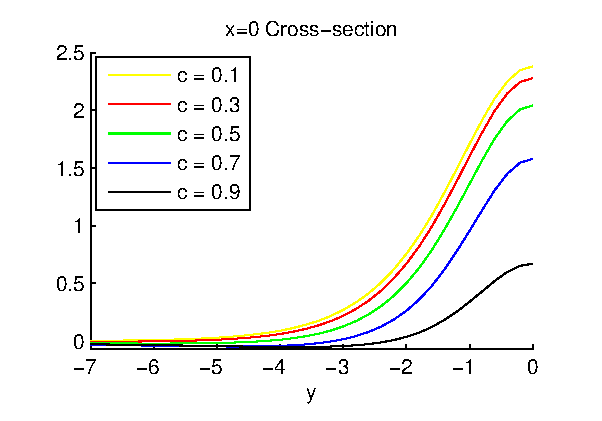
\includegraphics[width=\linewidth]{cross-sections/c=01__09beta=1x=0.eps}
	\end{minipage}	
	\begin{minipage}[b]{0.5\linewidth}
		\raggedright
		 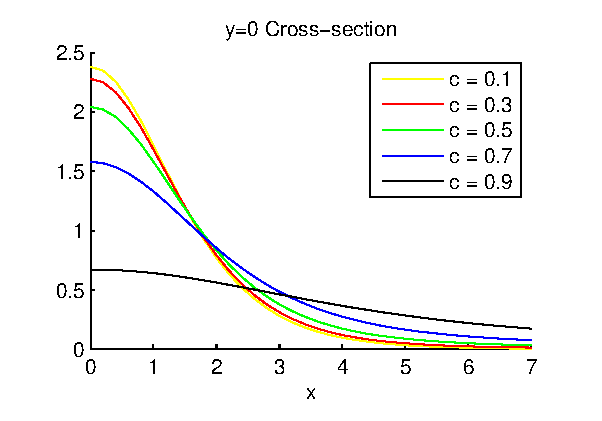
\includegraphics[width=\linewidth]{cross-sections/c=01__09beta=1y=0.eps}
	\end{minipage}
	\begin{minipage}[b]{0.5\linewidth}
		\raggedleft
		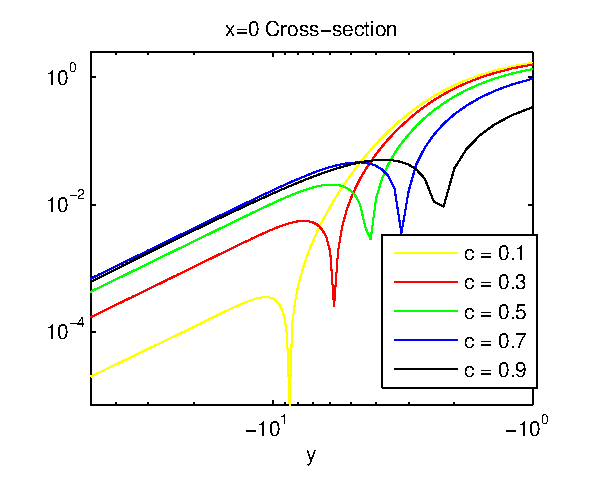
\includegraphics[width=\linewidth]{cross-sections/c=01__09beta=1Logx=0.eps}
	\end{minipage}	
	\begin{minipage}[b]{0.5\linewidth}
		\raggedright
		 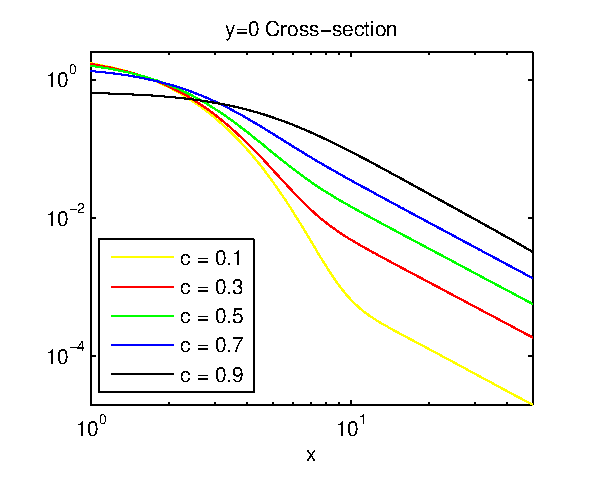
\includegraphics[width=\linewidth]{cross-sections/c=01__09beta=1Logy=0.eps}
	\end{minipage}
	\caption{Cross-sections of the numerical solution for $\beta=1$ and several  $c$}
	\label{profilesSpeedVarying}
\end{figure}

\begin{figure}[ht]
	\begin{minipage}[b]{0.5\linewidth}
		\raggedleft
		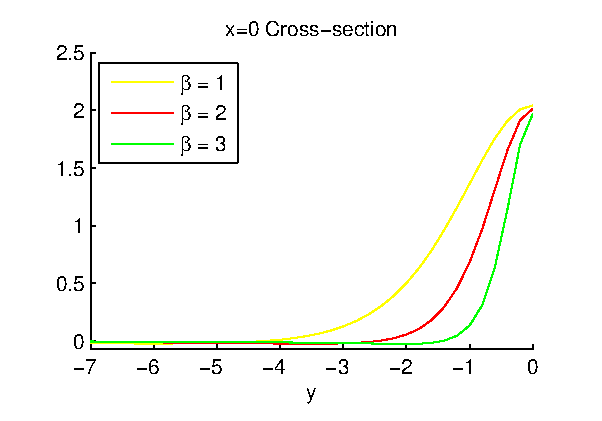
\includegraphics[width=\linewidth]{cross-sections/c=05beta=1__3x=0.eps}
	\end{minipage}	
	\begin{minipage}[b]{0.5\linewidth}
		\raggedright
		 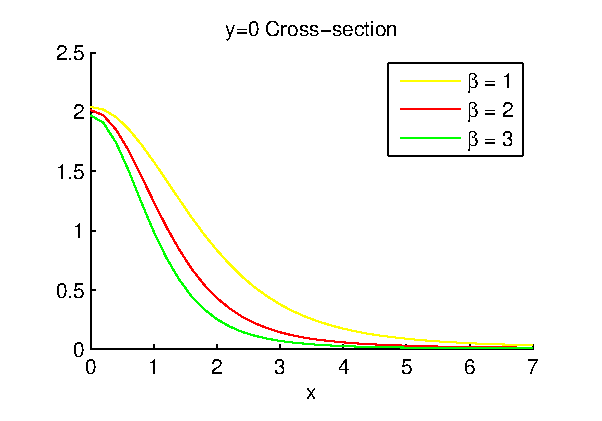
\includegraphics[width=\linewidth]{cross-sections/c=05beta=1__3y=0.eps}
	\end{minipage}
	\begin{minipage}[b]{0.5\linewidth}
		\raggedleft
		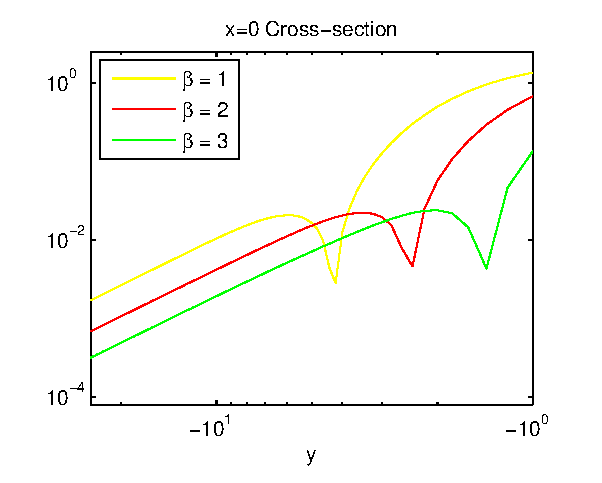
\includegraphics[width=\linewidth]{cross-sections/c=05beta=1__3Logx=0.eps}
	\end{minipage}	
	\begin{minipage}[b]{0.5\linewidth}
		\raggedright
		 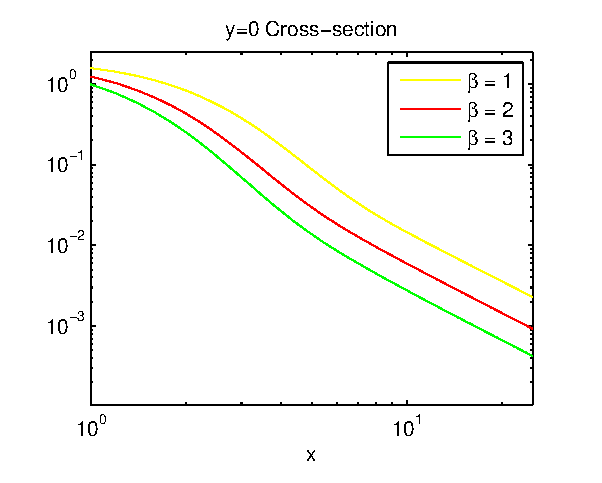
\includegraphics[width=\linewidth]{cross-sections/c=05beta=1__3Logy=0.eps}
	\end{minipage}
	\caption{Cross-sections of the numerical solution for $c=0.5$ and different $\beta$}
	\label{profilesBetaVarying}
\end{figure}

First, two aspects of the solution for different combinations of  $c$ and $\beta$   are plotted  on Figure~\ref{fig:solutions}. Both numerical solutions are computed on the  domain $\Omega = [0, 25]\times [0, 25]$ with $h = 0.1$ and then extended symmetrically to $ [-25, 25]\times [-25, 25]$. 
Only the essential part of the wave (near the center) is shown on these pictures. Top figures are level plots showing the waves from above and the bottom figures are 
three dimensional showing the structure of the wave in space. Very similar examples are presented on Figures~\ref{profilesSpeedVarying} and~\ref{profilesBetaVarying}, where $\Omega = [-50, 50]\times [-50, 50] $ and $h = 0.2$.


We perform a detailed study   of the numerical solution's shape with respect to main parameters -- the relative dispersion $\beta=\beta_1 / \beta_2$ and the velocity $c$.
 Figures~\ref{profilesSpeedVarying} and~\ref{profilesBetaVarying} show different aspects of the solution at $x=0$ and $y=0$ cross-sections. The parameter $\alpha$  is fixed as one ($\alpha = 1$) but  parameters $\beta $ and $c$ vary. We apply  the computational procedure with  $L_x = L_y = 50$, $h = 0.2$, $\epsilon = 1.0e-06$. 
On Figure~\ref{profilesSpeedVarying}, parameter $\beta=1$ is held constant and the wave dependence on the phase velocity  $c$ for $c=0.1, 0.3, 0.5, 0.7, 0.9$ is demonstrated.  Linear plots of the solution are presented on the upper row while  log-log plots of the absolute value of the solution are shown on the lower part.  These types of plots help us to establish the size of the computational box. 

One can observe that as the phase velocity $c$ increases the wave's support  along $x$ direction increases too, but the maximum of the wave decreases. The linear part of the solution on the log-log plots is under the governance of the boundary function.
Figure~\ref{profilesBetaVarying} presents the wave dependence on the dispersion parameter  $\beta=1, 2, 3$ with fixed
  phase velocity $c=0.5$. 
 One can see that the maximum of the wave slightly decreases as $\beta$ increases. The wave also becomes sharper along $x$ and $y$ directions.
The numerical results demonstrated on Figure~\ref{profilesSpeedVarying} and Figure~\ref{profilesBetaVarying} show very similar qualitative properties of the numerical solution obtained in  \cite{Ch2012} and by the numerical scheme in this paper.


\subsection{Comparison with best-fit formulae from \cite{Ch2011}} 


\begin{figure}[htbp]
	\begin{minipage}[b]{0.5\linewidth}
		\raggedleft
		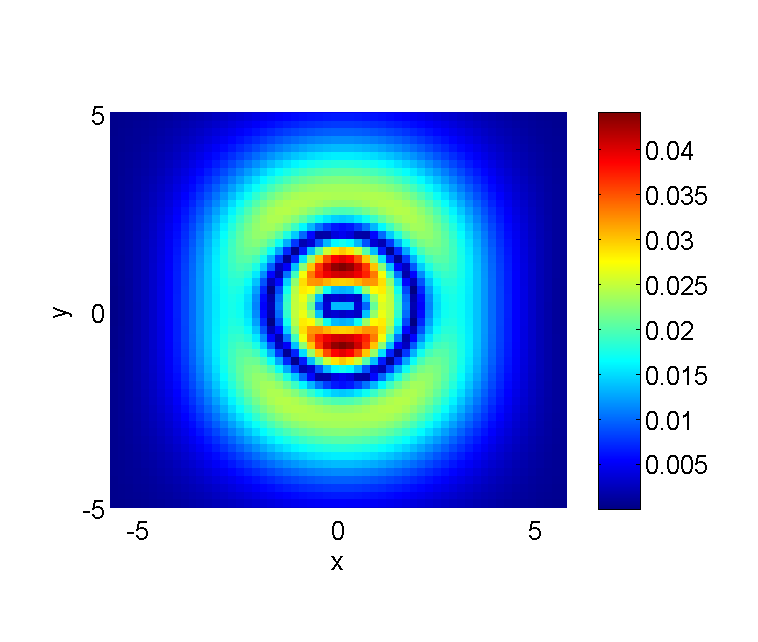
\includegraphics[width=\linewidth]{differences/difference_c=03_beta=1.eps}
	\end{minipage}
	\begin{minipage}[b]{0.5\linewidth}
		 \raggedright
		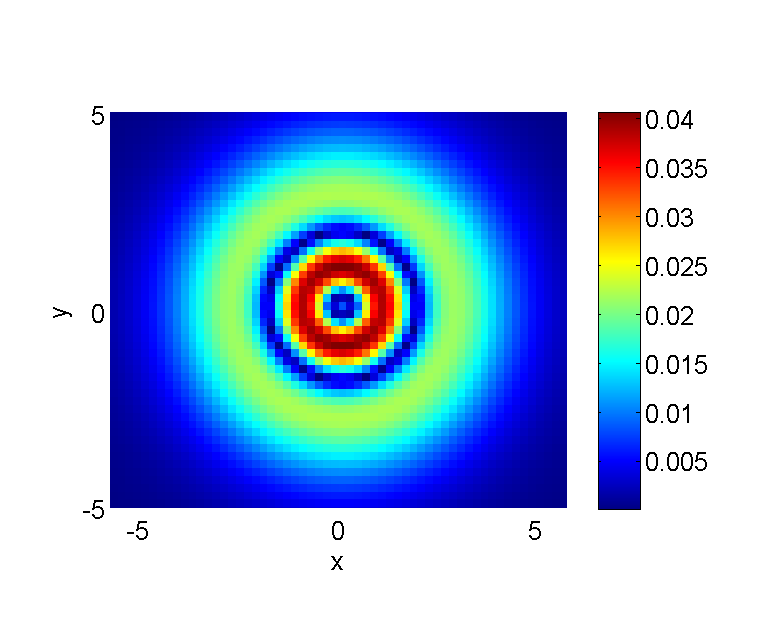
\includegraphics[width=\linewidth]{differences/difference_c=01_beta=1.eps}
	\end{minipage}
	\begin{minipage}[b]{0.5\linewidth}
		\raggedleft
		 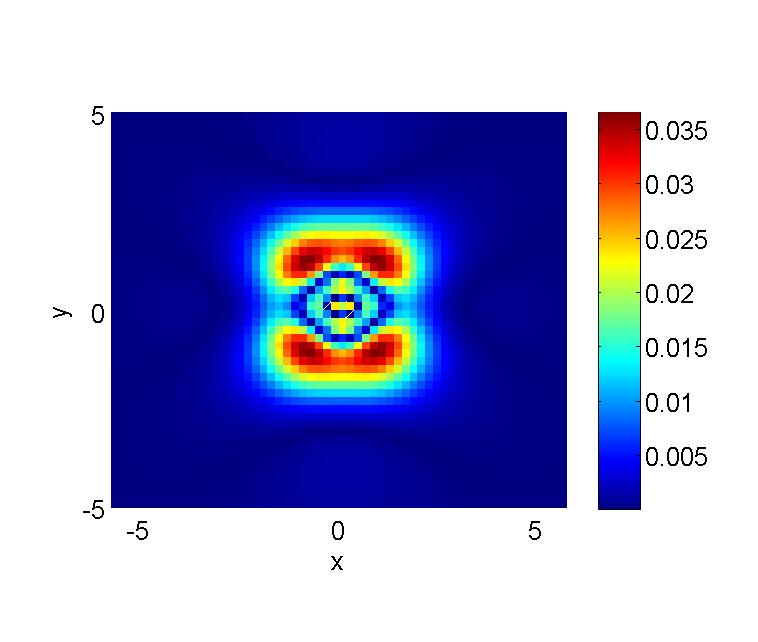
\includegraphics[width=\linewidth]{differences/difference_c=03_beta=3.eps}
	\end{minipage}
	\begin{minipage}[b]{0.5\linewidth}
		\raggedright
		 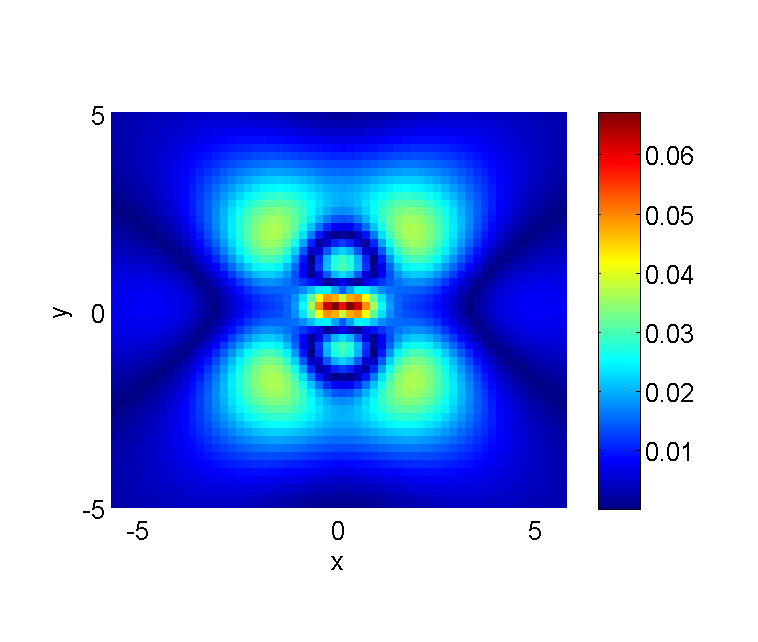
\includegraphics[width=\linewidth]{differences/difference_c=05_beta=1.eps}
	\end{minipage}
	\begin{minipage}[b]{0.5\linewidth}
		\raggedleft
		 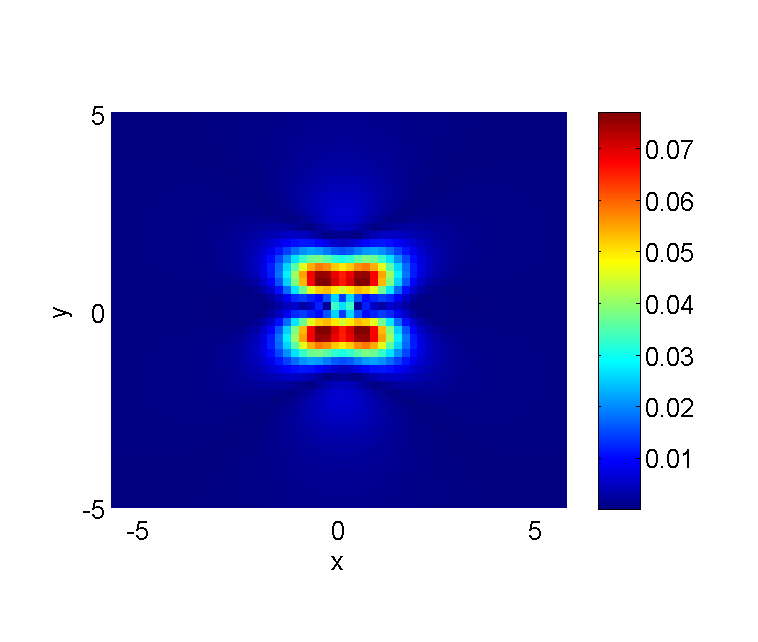
\includegraphics[width=\linewidth]{differences/difference_c=03_beta=5.eps}
		\centerline{$c=0.3$}
		\centerline{$\beta = 1,3,5$ (top to bottom) }
	\end{minipage}
	\begin{minipage}[b]{0.5\linewidth}
		\raggedright
		 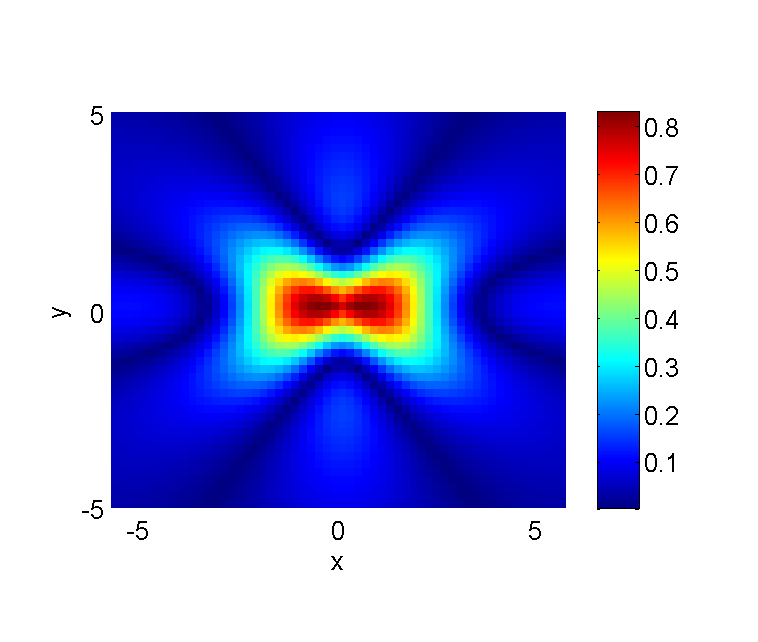
\includegraphics[width=\linewidth]{differences/difference_c=09_beta=1.eps}
		\centerline{$\beta = 1$}
		\centerline{$c = 0.1, 0.5, 0.9$ (top to bottom)}
	\end{minipage}
	\caption{Difference between the numerical solution $v$ and best fit  formulae $v^*$}
	\label{fig:difference}
\end{figure}
Figure~\ref{fig:difference} and Table~\ref{tab:first-der-t} demonstrate the  absolute value of the difference between  the solution $v^*$ by formulae \cite{Ch2011}  and the final solution of our procedure.

On the left side of Figure~\ref{fig:difference} the phase velocity $c = 0.3$ is fixed  and $\beta$ changes. On the right side  the dispersion parameter $\beta=1$ is kept constant while $c$ changes. The experiments are done on a $[-50,  50] \times [-50,50]$  domain  but only the results near the zero point are plotted. For each of the examples shown on Figure~\ref{fig:difference} more detailed estimate (using numbers) is given in Table~\ref{tab:first-der-t}. The difference is measured in the maximal and $L_2$ norms. One observes that for larger wave velocities $c$ and dispersion parameters $\beta$ the distinction becomes more pronounced. For example, for $\beta =1$ and $c=0.9$ the difference between the numerical solution obtained in this paper and the formulae  $v^*$ from \cite{Ch2011} becomes $\approx 0.8$ !

\begin{center}
\begin{table}[ht]
\centering
\resizebox{12cm}{!} {
		\begin{tabular}{|l|c|l l| c|l|c|l l|}
			\cline{1-4}\cline{6-9}
$\beta$&c&$\|v^*-v \|_{\infty }$&$\|v^*-v \|_{2 }$& &$\beta$& c&$\|v^*-v \|_{\infty }$&$\|v^*-v \|_{2 }$\\
			\cline{1-4}\cline{6-9}
1&     &4.4002e-02 & 1.4371e-01 & &    1& 0.1& 4.0554e-02  &1.4802e-01\\
3& 0.3 &3.6519e-02 & 9.0714e-02& &    1& 0.5& 6.7063e-02  &1.6766e-01\\
5&     &7.6927e-02 & 1.2936e-01 & &    1& 0.9&  8.2821e-01 &2.1671e0\\
			\cline{1-4}\cline{6-9}
\end{tabular}
}
		\caption{Differences between the numerical solution $v$ and best-fit solution $v^*$ from \cite{Ch2011}.}
\label{tab:first-der-t}
\end{table}
\end{center}

Figures~\ref{fig:c09beta1} and~\ref{fig:c05beta3} demonstrate  the sign of the  best-fit formulae $v^*$ and the  numerical solution $v$ obtained by the presented method.  The parameters of the problem are $\alpha = 1$, $\epsilon = 1.0e-06$, $h = 0.2$ and the  Laplacian is evaluated through 6th order finite differences. The colour bar is defined in the range $[-10.0e{-5},10.0e{-5}]$. Every value near the upper boundary and above  the interval is coloured in dark red and every value near the lower boundary and below - in dark blue.

One might notice that the solution has a very peculiar shape. There exist two curves which divide
the solution to 3 sub-domains: north and south domains, which are negative, and a middle, which is positive.
It is obvious that far away from the zero point the  solution $v(x,y)=v(r,\psi)$ obtained by this method always satisfies:
\begin{equation*}
\begin{split}
   & v(r,\psi)|_{\dO}
	 \left\{
	  \begin{array}{l l}
	    > 0 &  {\text{if}}\; \psi \in (-\phi , \phi  ) \cup (\pi-\phi ,\pi+ \phi ), \\ 
	    < 0 &  \text{if $\psi \in (\phi, \pi-\phi) \cup (\pi+\phi , -\phi ) $},  
	  \end{array} \right. \phi = \arccos( (2-c^2)^{-0.5})
\end{split}
\end{equation*}

and the   best-fit formula \cite{Ch2011} 
always satisfies:
\begin{equation*}
\begin{split}
   & v(r,\psi)|_{\dO}
	 \left\{
	  \begin{array}{l l}
	    > 0 &  \; {\text{if}}\; \psi \in (-\pi/4 , \pi/4  ) \cup (3\pi/4 ,5\pi/4   ), \\ 
	    < 0 &   \; \text{if $\psi \in (\pi/4, 3\pi/4) \cup (5\pi/4 , -\pi/4 ) $}.  
	  \end{array} \right.
\end{split}
\end{equation*}

\begin{figure}[htbp]
	\begin{minipage}[b]{0.45\linewidth}
		\raggedleft
		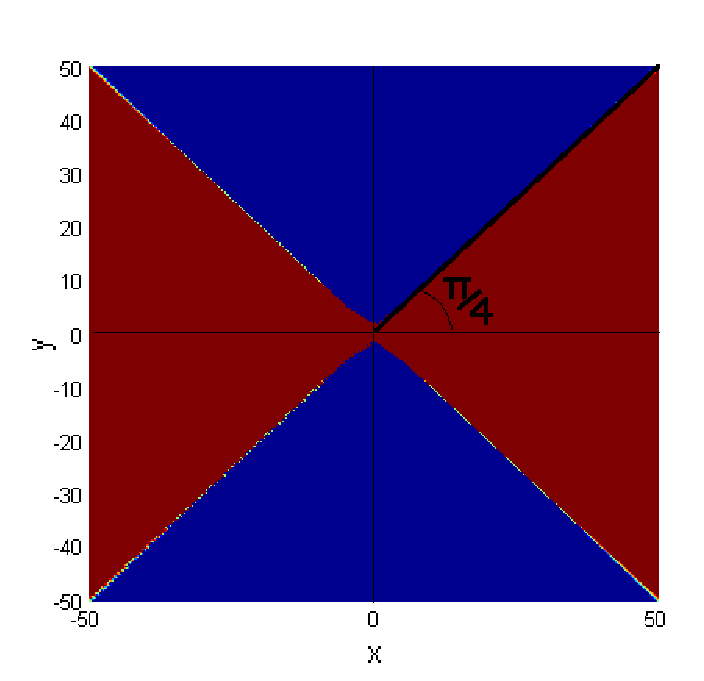
\includegraphics[width=\linewidth]{positiveNegativeDomains/IC_bnd50_c090_bt1.eps}
		\centerline{Solution  by formulae \cite{Ch2011}}
	\end{minipage}
	\begin{minipage}[b]{0.45\linewidth}
		 \raggedright
		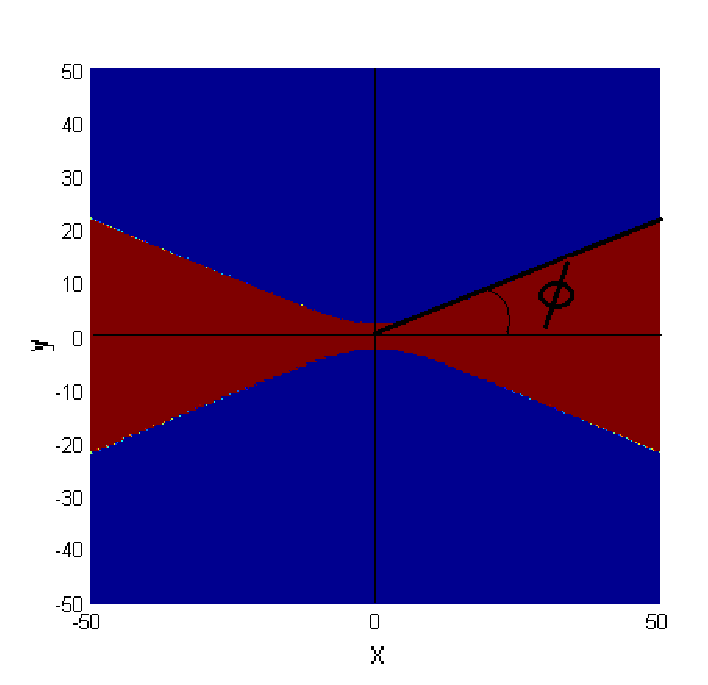
\includegraphics[width=\linewidth]{positiveNegativeDomains/SOL_bnd50_c090_bt1.eps}
		\centerline{Solution  by this method}
	\end{minipage}
	\caption{Sign of the solutions, $c=0.9$, $\beta = 1$}
	\label{fig:c09beta1}
\end{figure}

\begin{figure}[htbp]
	\begin{minipage}[b]{0.45\linewidth}
		\raggedleft
		\includegraphics[width=\linewidth]{positiveNegativeDomains/IC_bnd50_c050_bt3.eps}
		\centerline{Solution  by formulae \cite{Ch2011}}
	\end{minipage}
	\begin{minipage}[b]{0.45\linewidth}
		 \raggedright
		\includegraphics[width=\linewidth]{positiveNegativeDomains/SOL_bnd50_c050_bt3.eps}
		\centerline{Solution  by this method}
	\end{minipage}
	\caption{Sign of the solutions, $c=0.5$, $\beta = 3$}
	\label{fig:c05beta3}
\end{figure}

Notice that for smaller velocities $c \in [0, 0.57]$  the relation $\phi \in [\pi/4-\pi/30, \pi/4+\pi/30]$ holds for $\phi$. Recall the restriction $c \in min(1,1/\sqrt{\beta})$ made in the beginning of the paper. 
Thus larger $\beta$'s have impact on the velocity interval which reflects on the angle $\phi$ and thus on the positive/negative domain coverage. E.g. on Figure~\ref{fig:c05beta3} with $\beta = 3$, for the solution we have that $\phi \approx \pi/4$. 
But for $\beta = 1$ and $c=0.9$ (see Figure~\ref{fig:c09beta1}) there is a big difference between positive/negative parts of the solution obtained here and in \cite{Ch2011}! 
It is obvious that our solution $v$ and the best-fit  formulae $v^*$ from \cite{Ch2011} differ when compared to this characteristic - for some cases significantly, for others - slightly.

\section{Conclusion}
Fourth and sixth order finite difference schemes are applied for numerical evaluation of the travelling wave solutions to the Boussinesq equation in this paper. New conditions on the computational boundaries are devised. The high accuracy of the method applied is demonstrated on several experiments. The numerical solution obtained here performs similarly to the numerical solutions given in \cite{Ch2011,Ch2012} with respect to solution shape and the dependence on the velocity $c$ and relative dispersion $\beta$. 
The best-fit approximation formulae from  \cite{Ch2011} fail to satisfy the initial equation in the classical sense in the neighborhood of the origin. 
In the future, we will exploit the obtained numerical traveling wave solutions as initial data to the corresponding Boussinesq equation in order to seek two dimensional solitary wave solutions to \rf{eq1}.

\begin{thebibliography}{30}

\bibitem{chd-chr}
J.~Choudhury, C.~Christov, 2D  Solitary waves of  Boussinesq equation, CP75, (2005) 85–90.

\bibitem{cher}
A.~Chertock, C.~Christov, A.~Kurganov, Central-upwind schemes for the  Boussinesq paradigm equation, Comp. Sci. High Performance Comp. IV, NNFM, 113, (2011) 267–281.

\bibitem{chr-chr-07}
M.~Christou, C.~I.~Christov, Fourier–Galerkin method for 2D solitons of Boussinesq equation, 
Mathematics and Computers in Simulation 74 (2007) 82–92.
 
\bibitem{chr-chr}
M.~Christou, C.~I.~Christov, Galerkin Spectral Method for the 2D Solitary
Waves of Boussinesq Paradigm Equation, CP 1186 (2009) 217 -- 225.

\bibitem{Ch1996}
C.~I.~Cristov, Conservative difference scheme for Boussinesq model of
surface waves, Proc. ICFDS Oxford (1996) 343--349.

\bibitem{ChChr}
C.~I.~Christov, An energy-consistent dispersive shallow-water model,
Wave Motion,  34, (2001) 161 -- 174


\bibitem{Ch2011}
C.~I.~Christov, J. Choudhury, Perturbation solution  for the 2D Boussinesq equation,       
Mech. Res. Commun., 38 (2011)  274 -- 281.

\bibitem{Ch2012}
C.~I.~Christov,  Numerical implementation of the asymptotic boundary conditions
for steadily propagating 2D solitons of   Boussinesq type equation,       
Math. Computers  Simul., 82 (2012)  1079 -- 1092.

\bibitem{dani}
C.~Christov, N.~Kolkovska, D.~Vasileva, On the numerical simulation of unsteady solutions for the 2D Boussinesq paradigm equation, LNCS, 6046  (2011) 386 -- 394.

\bibitem{forn}
B.~Fornberg, Generation of Finite Difference Formulas on Arbitrarily Spaced Grids, 
Math. Comput., 51(1988),  699 -- 706.

\bibitem{sam}
A.~Samarskii, The theory of difference schemes, M. Dekker,  2001.


\end{thebibliography}


\end{document}
-----------------------------------------------------------------------------------------------------------------------------------


\bibitem{Ch2011}
A.~Chertock, C.~I.~Christov and A.~Kurganov,  Central-upwind schemes for
the Boussinesq paradigm equation, {\it Computational
Sci., \& High performance Computing IV, NNFM}, 113, 267--281 (2011).

  

\bibitem{Ch2009}
M.~Christou and C.~I.~ Christov, Galerkin spectral method for the 2D
solitary waves of Boussinesq paradigm equation,  \emph{AIP}
\textbf{1186}, 217 --224 (2009).

\bibitem{ChriTodoChri_AMiTaNS11}
 C.~I.~Christov, M.~D.~Todorov, M.~A.~Christou, Perturbation solution
for the 2D shallow-water waves, \emph{AIP Proceedings} 1404, 49-56,
(2011)

\bibitem{Chri2001_Vaj} C.~I.~Christov, In: \emph{Differential Equations
and Nonlinear Mechanics}, K. Vajravelu, ed., 63--77 (2001).


\bibitem{Ch1994}
C~I.~Christov and M.~Velarde, Inelastic interaction of Boussinesq
solutions, \emph{Intern. J Bifurcation Chaos}
\textbf{4}, 1095 -- 1112 (1994).


 \bibitem{nk-aip}
 N.~Kolkovska, M.~Dimova,
A New Conservative Finite Different Scheme for  Boussinesq Paradigm
Equation, CEJM (2011) DOI: 10.2478/s11533-012-0011-0


\bibitem{kutev}
Kutev N.,  Kolkovska N., Dimova M.,  Christov  C.I., Theoretical and
numerical aspects for global existence and
blow up for the solutions to Boussinesq paradigm equation,
AIP Conf. Proc. 1404 (2011) 68--76

 